\documentclass[floatsintext,man]{apa6}

\usepackage{amssymb,amsmath}
\usepackage{ifxetex,ifluatex}
\usepackage{fixltx2e} % provides \textsubscript
\ifnum 0\ifxetex 1\fi\ifluatex 1\fi=0 % if pdftex
  \usepackage[T1]{fontenc}
  \usepackage[utf8]{inputenc}
\else % if luatex or xelatex
  \ifxetex
    \usepackage{mathspec}
    \usepackage{xltxtra,xunicode}
  \else
    \usepackage{fontspec}
  \fi
  \defaultfontfeatures{Mapping=tex-text,Scale=MatchLowercase}
  \newcommand{\euro}{€}
\fi
% use upquote if available, for straight quotes in verbatim environments
\IfFileExists{upquote.sty}{\usepackage{upquote}}{}
% use microtype if available
\IfFileExists{microtype.sty}{\usepackage{microtype}}{}

% Table formatting
\usepackage{longtable, booktabs}
\usepackage{lscape}
% \usepackage[counterclockwise]{rotating}   % Landscape page setup for large tables
\usepackage{multirow}		% Table styling
\usepackage{tabularx}		% Control Column width
\usepackage[flushleft]{threeparttable}	% Allows for three part tables with a specified notes section
\usepackage{threeparttablex}            % Lets threeparttable work with longtable

% Create new environments so endfloat can handle them
% \newenvironment{ltable}
%   {\begin{landscape}\begin{center}\begin{threeparttable}}
%   {\end{threeparttable}\end{center}\end{landscape}}

\newenvironment{lltable}
  {\begin{landscape}\begin{center}\begin{ThreePartTable}}
  {\end{ThreePartTable}\end{center}\end{landscape}}




% The following enables adjusting longtable caption width to table width
% Solution found at http://golatex.de/longtable-mit-caption-so-breit-wie-die-tabelle-t15767.html
\makeatletter
\newcommand\LastLTentrywidth{1em}
\newlength\longtablewidth
\setlength{\longtablewidth}{1in}
\newcommand\getlongtablewidth{%
 \begingroup
  \ifcsname LT@\roman{LT@tables}\endcsname
  \global\longtablewidth=0pt
  \renewcommand\LT@entry[2]{\global\advance\longtablewidth by ##2\relax\gdef\LastLTentrywidth{##2}}%
  \@nameuse{LT@\roman{LT@tables}}%
  \fi
\endgroup}


\ifxetex
  \usepackage[setpagesize=false, % page size defined by xetex
              unicode=false, % unicode breaks when used with xetex
              xetex]{hyperref}
\else
  \usepackage[unicode=true]{hyperref}
\fi
\hypersetup{breaklinks=true,
            pdfauthor={},
            pdftitle={Supplementary Materials: Early language experience in a Tseltal Mayan village},
            colorlinks=true,
            citecolor=blue,
            urlcolor=blue,
            linkcolor=black,
            pdfborder={0 0 0}}
\urlstyle{same}  % don't use monospace font for urls

\setlength{\parindent}{0pt}
%\setlength{\parskip}{0pt plus 0pt minus 0pt}

\setlength{\emergencystretch}{3em}  % prevent overfull lines


% Manuscript styling
\captionsetup{font=singlespacing,justification=justified}
\usepackage{csquotes}
\usepackage{upgreek}

 % Line numbering
  \usepackage{lineno}
  \linenumbers


\usepackage{tikz} % Variable definition to generate author note

% fix for \tightlist problem in pandoc 1.14
\providecommand{\tightlist}{%
  \setlength{\itemsep}{0pt}\setlength{\parskip}{0pt}}

% Essential manuscript parts
  \title{Supplementary Materials: Early language experience in a Tseltal Mayan
village}

  \shorttitle{Supp. Materials: Early language in a Tseltal village}


  \author{Marisa Casillas\textsuperscript{1}, Penelope Brown\textsuperscript{1}, \& Stephen C. Levinson\textsuperscript{1}}

  % \def\affdep{{"", "", ""}}%
  % \def\affcity{{"", "", ""}}%

  \affiliation{
    \vspace{0.5cm}
          \textsuperscript{1} Max Planck Institute for Psycholinguistics  }

  \authornote{
    Correspondence concerning this article should be addressed to Marisa
    Casillas, P.O. Box 310, 6500 AH Nijmegen, The Netherlands. E-mail:
    \href{mailto:Marisa.Casillas@mpi.nl}{\nolinkurl{Marisa.Casillas@mpi.nl}}
  }


  



  \usepackage{float}
  \floatplacement{figure}{H}
  \usepackage{placeins}

\usepackage{amsthm}
\newtheorem{theorem}{Theorem}[section]
\newtheorem{lemma}{Lemma}[section]
\theoremstyle{definition}
\newtheorem{definition}{Definition}[section]
\newtheorem{corollary}{Corollary}[section]
\newtheorem{proposition}{Proposition}[section]
\theoremstyle{definition}
\newtheorem{example}{Example}[section]
\theoremstyle{definition}
\newtheorem{exercise}{Exercise}[section]
\theoremstyle{remark}
\newtheorem*{remark}{Remark}
\newtheorem*{solution}{Solution}
\begin{document}

\maketitle

\setcounter{secnumdepth}{0}



\section{Full model outputs}\label{models}

In the main text we only report \emph{significant} effects on two speech
environment variables: TCDS min/hr and ODS min/hr. Here in the
Supplementary Materials we give the full model output tables for each
analysis, including re-leveled versions of each model to show all three
of the two-way contrasts between the three-level time-of-day factor
(i.e., morning vs.~midday, morning vs.~afternoon, and midday
vs.~afternoon). We also include, for each of the measures, a histogram
showing how each variable is distributed (i.e., because they are
non-normal and/or zero-inflated) and a figure showing the distribution
of model residuals. For every negative binomial model, we also include
the full model output table and residual plots for matching gaussian
mixed-effects regressions which uses a logged dependent measure. Such
gaussian models with logged measures are an alternative solution to
analyzing non-normal distributions sometimes used in psycholinguistics,
but are not suitable for the current data given how our speech
environment measures are distributed, particularly in the randomly
sampled clips (see, e.g., Figures \protect\hyperlink{fig1}{1},
\protect\hyperlink{fig7}{7}, \protect\hyperlink{fig10}{10},
\protect\hyperlink{fig13}{13}, \protect\hyperlink{fig19}{19}). Overall,
however, the gaussian models show a qualitatively similar pattern of
results. None of the gaussian model results are presented in the main
text---only here as supplementary information.

\subsection{How to interpret the model
output}\label{how-to-interpret-the-model-output}

All models were run with the glmm-TMB library in R (Brooks et al.,
2017a, 2017b). Note that, in the negative binomial regressions, the
dependent variables have been rounded to the nearest integer (e.g., 3.2
minutes of TCDS per hour becomes 3 minutes per hour in the model).

The predictors in the models are abbreviated as follows: tchiyr.std =
centered, standardized target child age in months; stthr.tri = the start
time of the clip as either morning, midday, or afternoon; hsz.std =
centered, standardized household size of the target child; nsk.std =
centered, standardized number of speakers present in the clip,
aclew\_child\_id = the unique identifier for each child. The predictors
are sometimes combined in two-way interactions, as shown below with a
\enquote{:} separator between predictor names (e.g., tchiyr.std:nsk.std
= a two-way interaction of target child age and number of speakers
present).

In each model output table, the \enquote{component} shows what kind of
model the estimate derives from (e.g., the zero-inflated models include
both a conditional \enquote{cond} set of predictors, random effects, and
zero-inflation \enquote{zi} predictors). The \enquote{term} is the
estimated predictor. The \enquote{statistic} is the estimated
\emph{z}-statistic for each predictor's effect. The other labels are
self-explanatory.

As more data are added to this corpus, the analyses will also be
updated, as will this supplementary model information, all of which will
be available online at:
\url{https://middycasillas.shinyapps.io/Tseltal_Child_Language_Environment/}.

\subsection{Target-child-directed speech (TCDS)}\label{models-tcds}

\subsubsection{Random clips}\label{models-tcds-random}

TCDS rate in the random clips demonstrated a skewed distribution with
extra cases of zero \protect\hyperlink{fig1}{Figure 1}. We therefore
modeled it using a zero-inflated negative binomial mixed-effects
regression in the main text: results for the two models demonstrating
all pairwise effects of time of day are shown in
\protect\hyperlink{tab1}{Table 1} and \protect\hyperlink{tab2}{Table 2}.
The residuals for the default model (\protect\hyperlink{tab1}{Table 1})
are shown in \protect\hyperlink{fig2}{Figure 2}.

\FloatBarrier

\begin{figure}[H]

{\centering 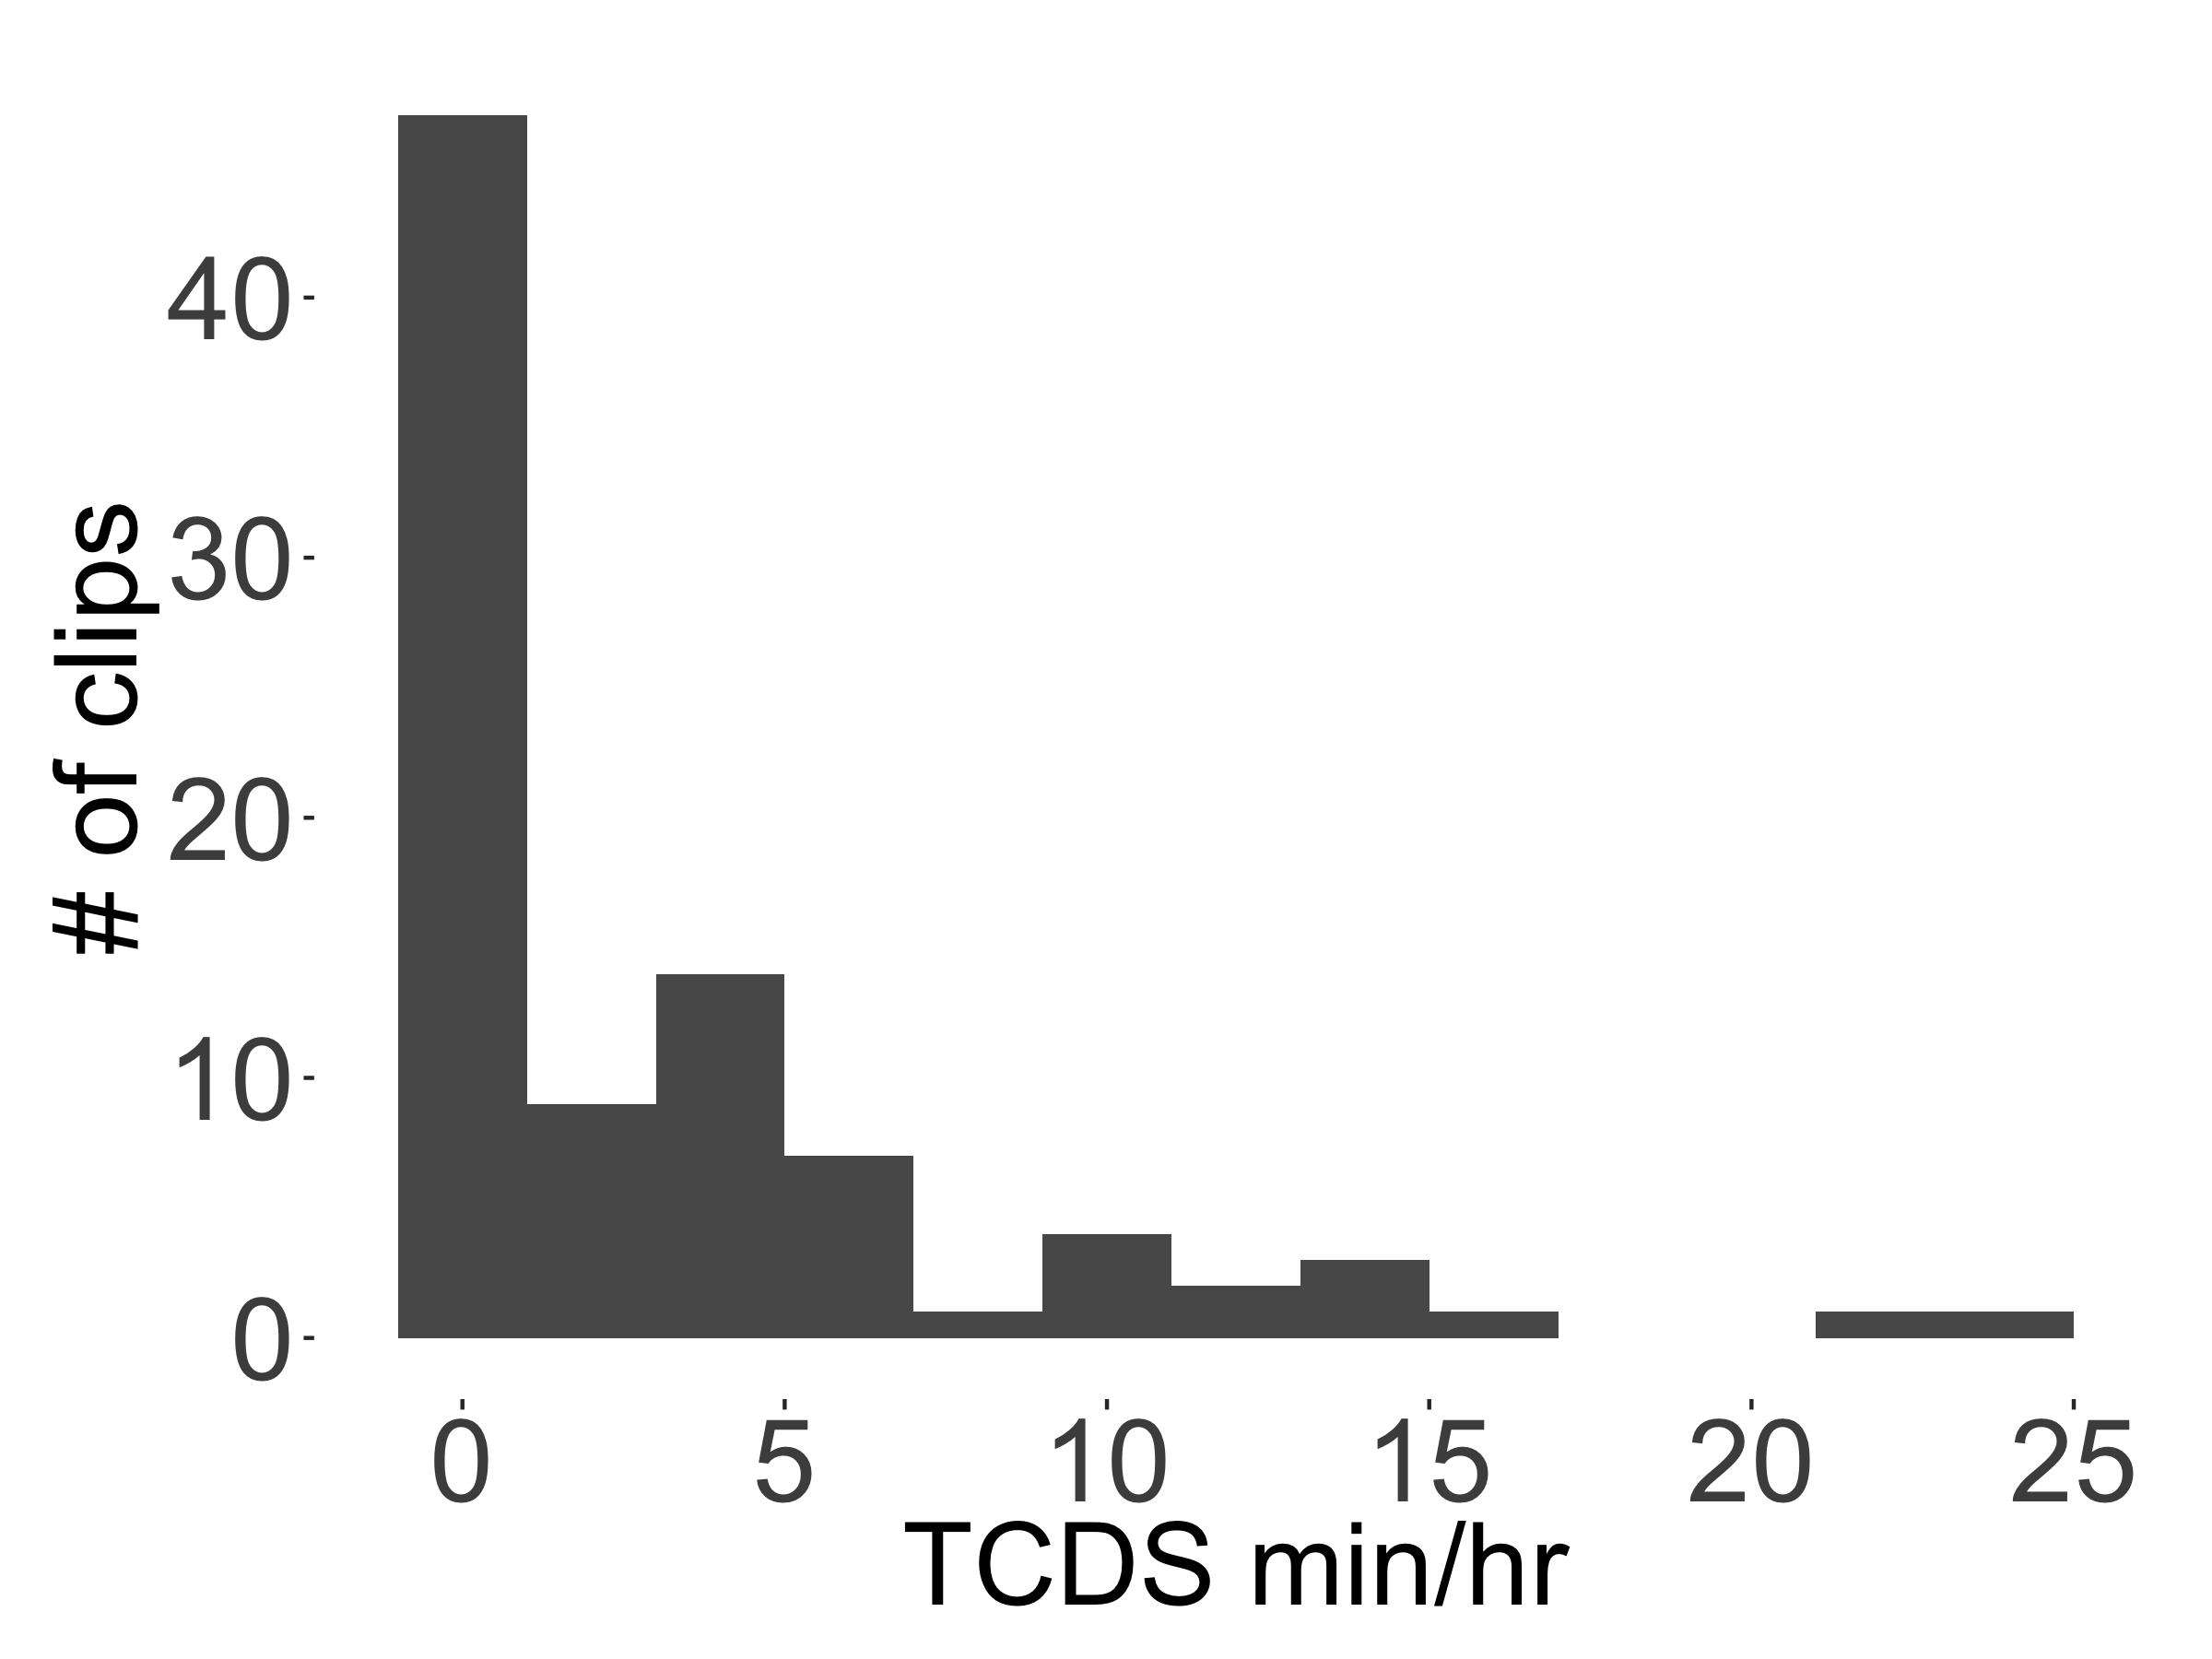
\includegraphics[width=0.4\linewidth]{www/TCDS_random_distribution} 

}

\caption{The distribution of TCDS rates found across the 90 random clips.}\label{fig:fig1}
\end{figure}

\FloatBarrier

\begin{table}[tbp]
\begin{center}
\begin{threeparttable}
\caption{\label{tab:tab1}Full output of the zero-inflated negative binomial mixed-effects regression of TCDS min/hr for the random sample, with midday as the reference level for time of day.}
\begin{tabular}{llllll}
\toprule
component & \multicolumn{1}{c}{term} & \multicolumn{1}{c}{estimate} & \multicolumn{1}{c}{std.error} & \multicolumn{1}{c}{statistic} & \multicolumn{1}{c}{p.value}\\
\midrule
cond & (Intercept) & 0.91 & 0.36 & 2.53 & 0.01\\
cond & tchiyr.std & 0.60 & 0.36 & 1.68 & 0.09\\
cond & stthr.trimorning & 0.83 & 0.40 & 2.09 & 0.04\\
cond & stthr.triafternoon & 0.49 & 0.37 & 1.31 & 0.19\\
cond & hsz.std & 0.01 & 0.22 & 0.04 & 0.97\\
cond & nsk.std & -0.12 & 0.16 & -0.75 & 0.45\\
cond & tchiyr.std:stthr.trimorning & -0.28 & 0.39 & -0.73 & 0.47\\
cond & tchiyr.std:stthr.triafternoon & -0.85 & 0.38 & -2.26 & 0.02\\
cond & tchiyr.std:nsk.std & 0.57 & 0.19 & 2.95 & 0.00\\
zi & (Intercept) & -57.43 & 15,426.18 & 0.00 & 1.00\\
zi & nsk.std & -55.68 & 15,691.06 & 0.00 & 1.00\\
random\_effect & aclew\_child\_id & 0.31 & NA & NA & NA\\
\bottomrule
\end{tabular}
\end{threeparttable}
\end{center}
\end{table}

\begin{table}[tbp]
\begin{center}
\begin{threeparttable}
\caption{\label{tab:tab2}Model output of the zero-inflated negative binomial mixed-effects regression of TCDS min/hr for the random sample, with afternoon as the reference level for time of day.}
\begin{tabular}{llllll}
\toprule
component & \multicolumn{1}{c}{term} & \multicolumn{1}{c}{estimate} & \multicolumn{1}{c}{std.error} & \multicolumn{1}{c}{statistic} & \multicolumn{1}{c}{p.value}\\
\midrule
cond & (Intercept) & 1.40 & 0.22 & 6.47 & 0.00\\
cond & tchiyr.std & -0.25 & 0.25 & -1.02 & 0.31\\
cond & stthr.tri.amidday & -0.49 & 0.37 & -1.31 & 0.19\\
cond & stthr.tri.amorning & 0.34 & 0.27 & 1.26 & 0.21\\
cond & hsz.std & 0.01 & 0.22 & 0.04 & 0.97\\
cond & nsk.std & -0.12 & 0.16 & -0.75 & 0.45\\
cond & tchiyr.std:stthr.tri.amidday & 0.85 & 0.38 & 2.26 & 0.02\\
cond & tchiyr.std:stthr.tri.amorning & 0.57 & 0.30 & 1.90 & 0.06\\
cond & tchiyr.std:nsk.std & 0.57 & 0.19 & 2.95 & 0.00\\
zi & (Intercept) & -57.88 & 16,902.92 & 0.00 & 1.00\\
zi & nsk.std & -56.14 & 17,193.15 & 0.00 & 1.00\\
random\_effect & aclew\_child\_id & 0.31 & NA & NA & NA\\
\bottomrule
\end{tabular}
\end{threeparttable}
\end{center}
\end{table}

\FloatBarrier

\begin{figure}[H]

{\centering 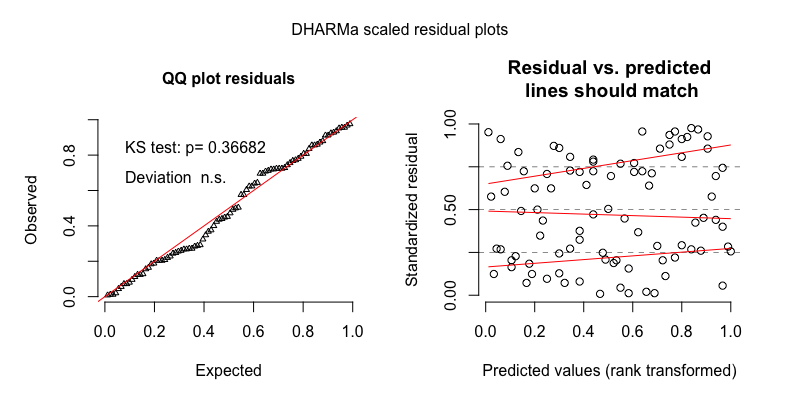
\includegraphics[width=0.9\linewidth]{www/TCDS_random_z-inb_res_plot} 

}

\caption{The model residuals from the zero-inflated negative binomial mixed-effects regression of TCDS min/hr for the random sample.}\label{fig:fig2}
\end{figure}

As an alternative analysis we generated parallel models of TCDS rate in
the random clips using gaussian mixed-effects regression with logged
values of TCDS: results for the two models demonstrating all pairwise
effects of time of day are shown in \protect\hyperlink{tab3}{Table 3}
and \protect\hyperlink{tab4}{Table 4}. The residuals for the default
gaussian model (\protect\hyperlink{tab3}{Table 3}) are shown in
\protect\hyperlink{fig3}{Figure 3}.

\FloatBarrier

\begin{table}[tbp]
\begin{center}
\begin{threeparttable}
\caption{\label{tab:tab3}Full output of the gaussian mixed-effects regression of TCDS min/hr for the random sample, with midday as the reference level for time of day.}
\begin{tabular}{llllll}
\toprule
component & \multicolumn{1}{c}{term} & \multicolumn{1}{c}{estimate} & \multicolumn{1}{c}{std.error} & \multicolumn{1}{c}{statistic} & \multicolumn{1}{c}{p.value}\\
\midrule
cond & (Intercept) & 0.82 & 0.19 & 4.33 & 0.00\\
cond & tchiyr.std & 0.54 & 0.22 & 2.42 & 0.02\\
cond & stthr.trimorning & 0.50 & 0.25 & 2.02 & 0.04\\
cond & stthr.triafternoon & 0.29 & 0.22 & 1.31 & 0.19\\
cond & hsz.std & -0.16 & 0.16 & -0.99 & 0.32\\
cond & nsk.std & 0.23 & 0.12 & 1.93 & 0.05\\
cond & tchiyr.std:stthr.trimorning & -0.17 & 0.27 & -0.65 & 0.52\\
cond & tchiyr.std:stthr.triafternoon & -0.68 & 0.24 & -2.85 & 0.00\\
cond & tchiyr.std:nsk.std & 0.23 & 0.14 & 1.66 & 0.10\\
random\_effect & aclew\_child\_id & 0.21 & NA & NA & NA\\
random\_effect & Residual & 0.84 & NA & NA & NA\\
\bottomrule
\end{tabular}
\end{threeparttable}
\end{center}
\end{table}

\begin{table}[tbp]
\begin{center}
\begin{threeparttable}
\caption{\label{tab:tab4}Model output of the gaussian mixed-effects regression of TCDS min/hr for the random sample, with afternoon as the reference level for time of day.}
\begin{tabular}{llllll}
\toprule
component & \multicolumn{1}{c}{term} & \multicolumn{1}{c}{estimate} & \multicolumn{1}{c}{std.error} & \multicolumn{1}{c}{statistic} & \multicolumn{1}{c}{p.value}\\
\midrule
cond & (Intercept) & 1.11 & 0.15 & 7.55 & 0.00\\
cond & tchiyr.std & -0.14 & 0.18 & -0.80 & 0.42\\
cond & stthr.tri.amidday & -0.29 & 0.22 & -1.31 & 0.19\\
cond & stthr.tri.amorning & 0.22 & 0.22 & 0.98 & 0.33\\
cond & hsz.std & -0.16 & 0.16 & -0.99 & 0.32\\
cond & nsk.std & 0.23 & 0.12 & 1.93 & 0.05\\
cond & tchiyr.std:stthr.tri.amidday & 0.68 & 0.24 & 2.85 & 0.00\\
cond & tchiyr.std:stthr.tri.amorning & 0.51 & 0.23 & 2.21 & 0.03\\
cond & tchiyr.std:nsk.std & 0.23 & 0.14 & 1.66 & 0.10\\
random\_effect & aclew\_child\_id & 0.21 & NA & NA & NA\\
random\_effect & Residual & 0.84 & NA & NA & NA\\
\bottomrule
\end{tabular}
\end{threeparttable}
\end{center}
\end{table}

\FloatBarrier

\begin{figure}[H]

{\centering 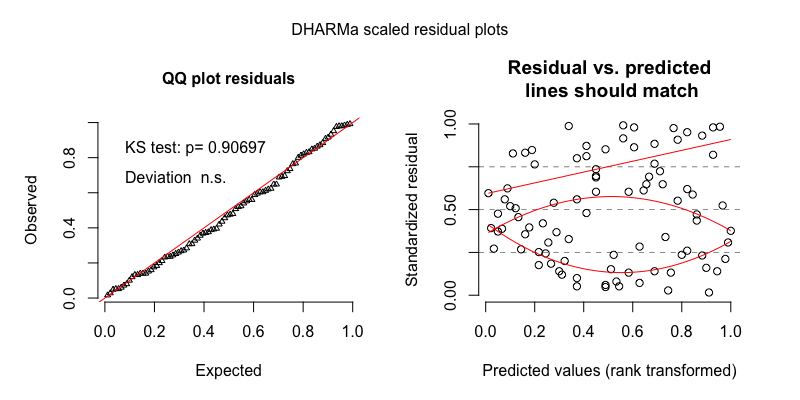
\includegraphics[width=0.9\linewidth]{www/TCDS_random_log_gaus_res_plot} 

}

\caption{The model residuals from the gaussian mixed-effects regression of TCDS min/hr for the random sample.}\label{fig:fig3}
\end{figure}

\FloatBarrier

\subsubsection{Turn-taking clips}\label{models-tcds-turntaking}

TCDS rate in the turn-taking clips demonstrated a slightly skewed, but
unimodal distribution \protect\hyperlink{fig4}{Figure 4}. We therefore
modeled it using a plain (i.e., non-zero-inflated) negative binomial
mixed-effects regression in the main text: results for the two models
demonstrating all pairwise effects of time of day are shown in
\protect\hyperlink{tab5}{Table 5} and \protect\hyperlink{tab6}{Table 6}.
The residuals for the default model (\protect\hyperlink{tab5}{Table 5})
are shown in \protect\hyperlink{fig5}{Figure 5}.

\FloatBarrier

\begin{figure}[H]

{\centering 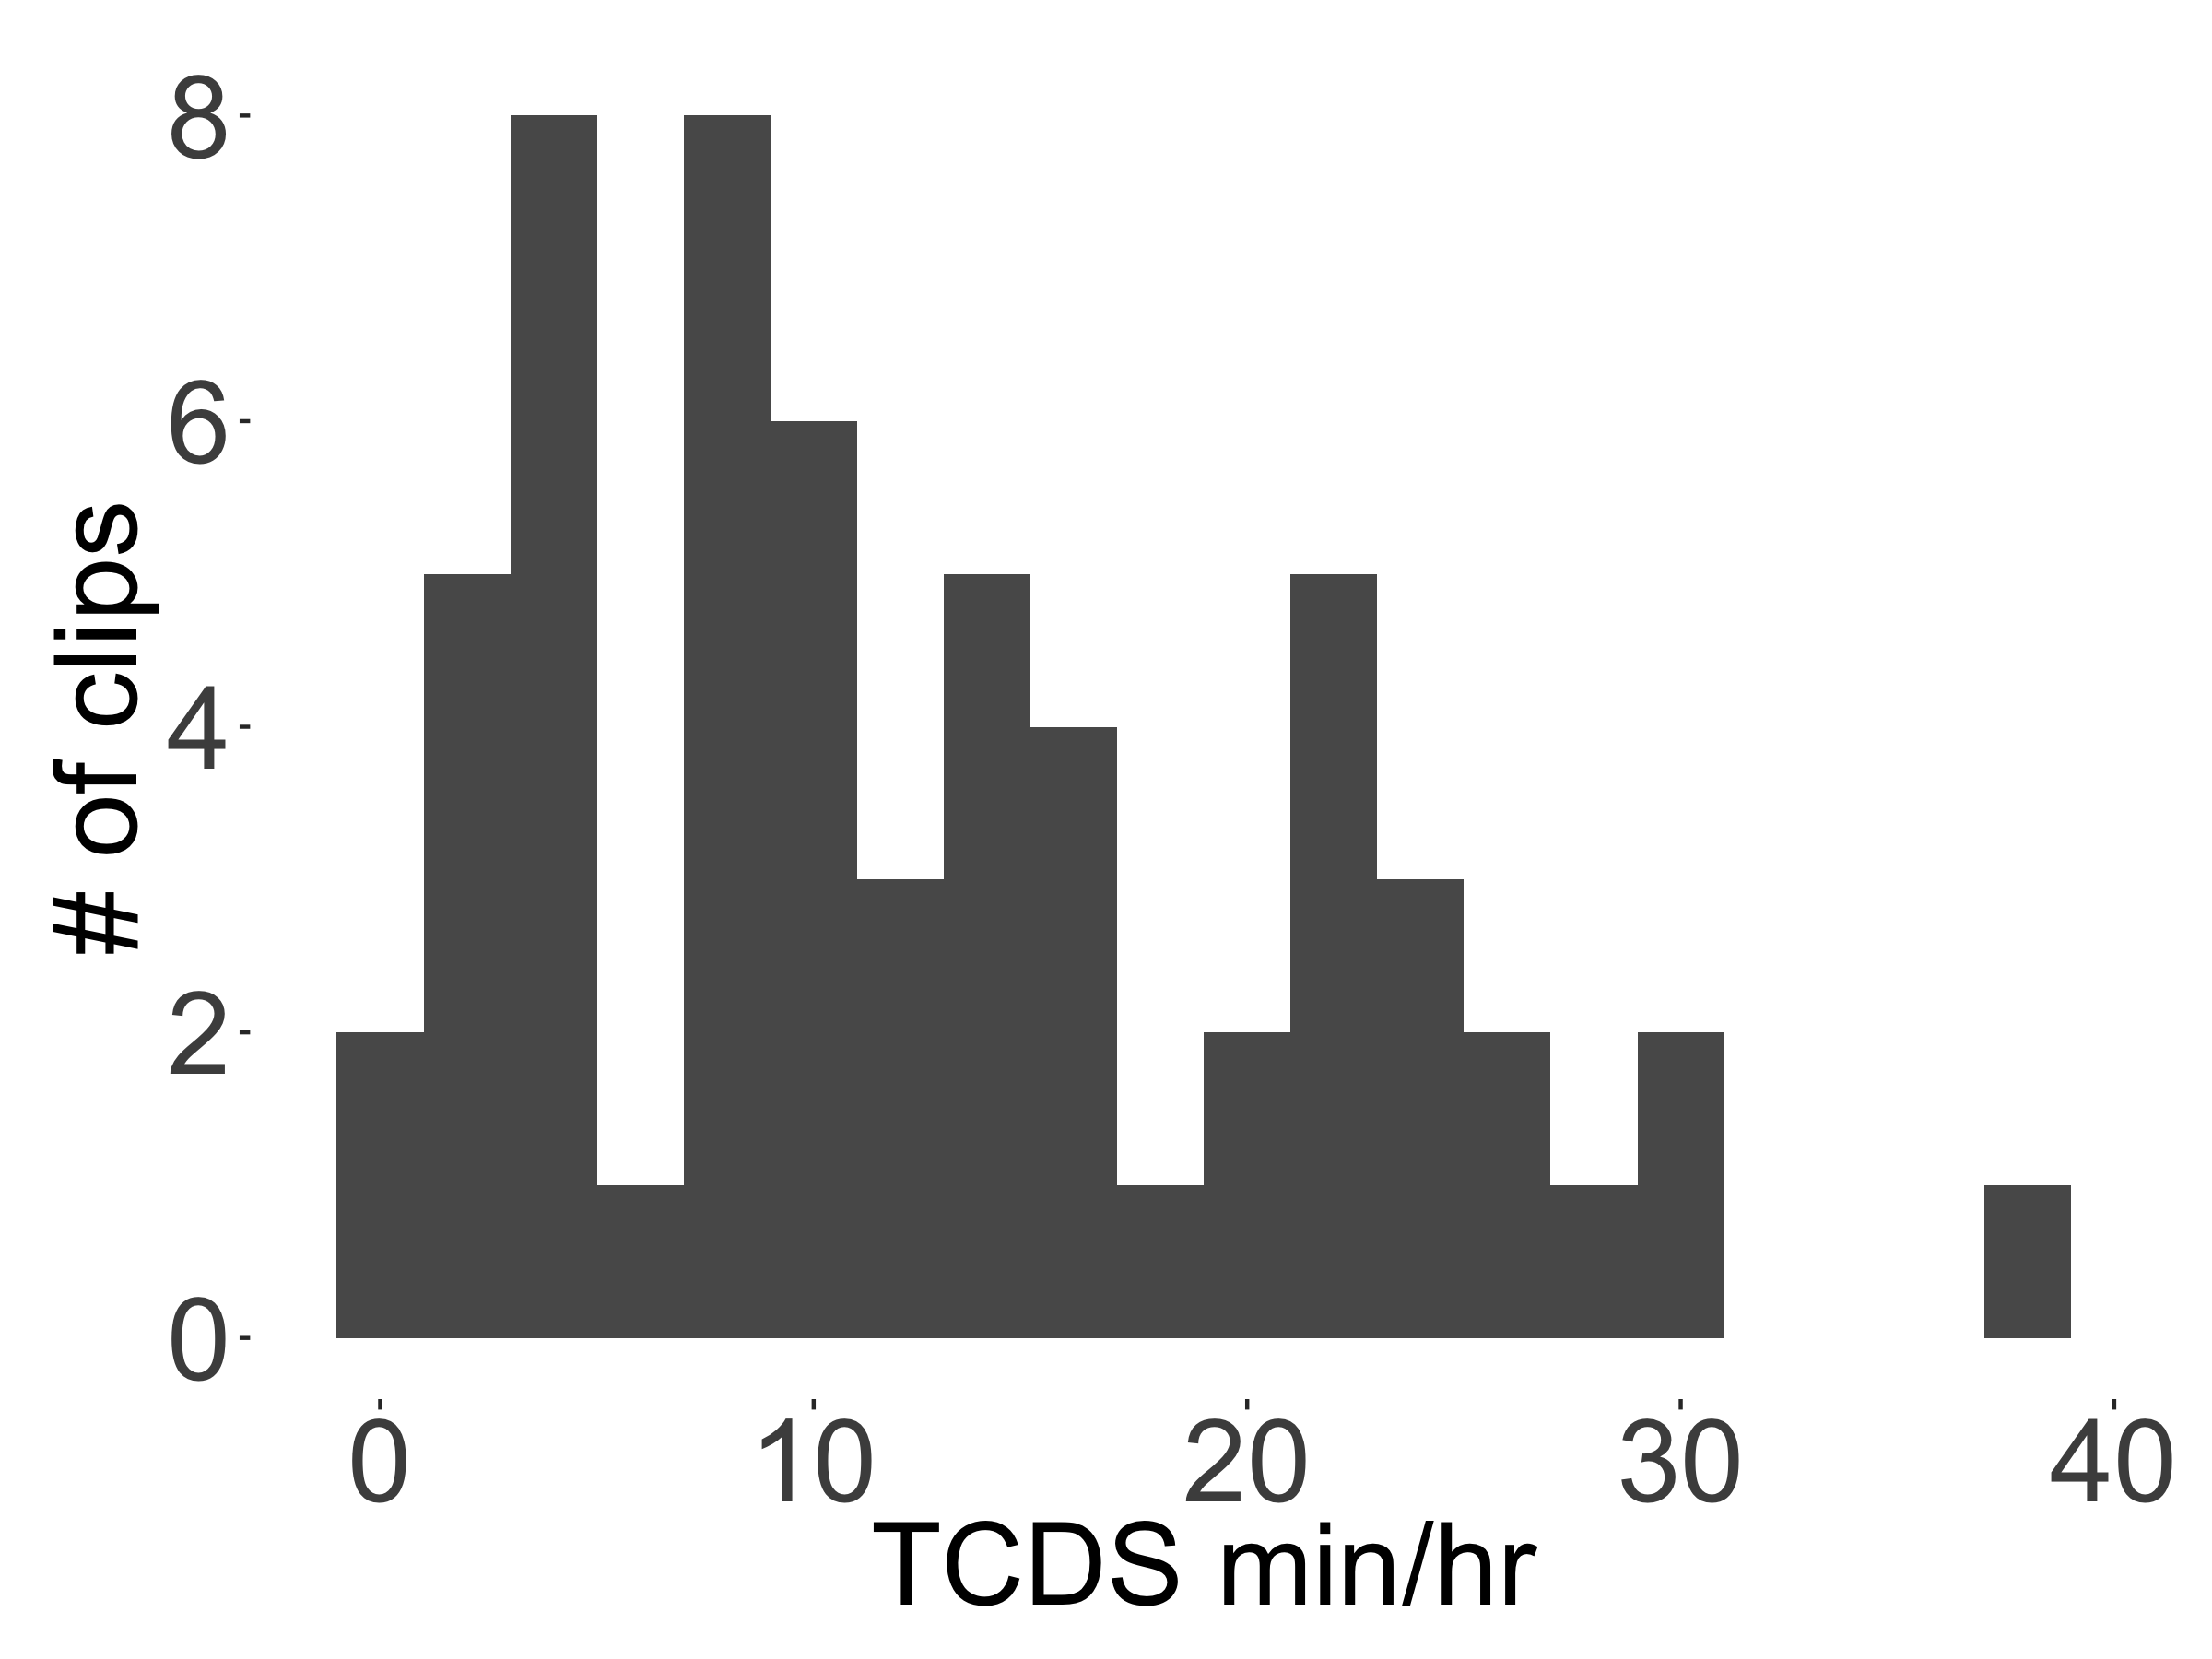
\includegraphics[width=0.4\linewidth]{www/TCDS_turntaking_distribution} 

}

\caption{The distribution of TCDS rates found across the 59 turn-taking clips.}\label{fig:fig4}
\end{figure}

\FloatBarrier

\begin{table}[tbp]
\begin{center}
\begin{threeparttable}
\caption{\label{tab:tab5}Full output of the negative binomial mixed-effects regression of TCDS min/hr for the turn-taking sample, with midday as the reference level for time of day.}
\begin{tabular}{llllll}
\toprule
component & \multicolumn{1}{c}{term} & \multicolumn{1}{c}{estimate} & \multicolumn{1}{c}{std.error} & \multicolumn{1}{c}{statistic} & \multicolumn{1}{c}{p.value}\\
\midrule
cond & (Intercept) & 2.52 & 0.22 & 11.32 & 0.00\\
cond & tchiyr.std & 0.08 & 0.21 & 0.38 & 0.70\\
cond & stthr.trimorning & 0.14 & 0.29 & 0.48 & 0.63\\
cond & stthr.triafternoon & 0.06 & 0.27 & 0.23 & 0.82\\
cond & hsz.std & 0.12 & 0.14 & 0.86 & 0.39\\
cond & nsk.std & -0.13 & 0.10 & -1.23 & 0.22\\
cond & tchiyr.std:stthr.trimorning & -0.13 & 0.29 & -0.47 & 0.64\\
cond & tchiyr.std:stthr.triafternoon & 0.00 & 0.24 & 0.01 & 1.00\\
cond & tchiyr.std:nsk.std & 0.06 & 0.13 & 0.46 & 0.65\\
random\_effect & aclew\_child\_id & 0.19 & NA & NA & NA\\
\bottomrule
\end{tabular}
\end{threeparttable}
\end{center}
\end{table}

\begin{table}[tbp]
\begin{center}
\begin{threeparttable}
\caption{\label{tab:tab6}Model output of the negative binomial mixed-effects regression of TCDS min/hr for the turn-taking sample, with afternoon as the reference level for time of day.}
\begin{tabular}{llllll}
\toprule
component & \multicolumn{1}{c}{term} & \multicolumn{1}{c}{estimate} & \multicolumn{1}{c}{std.error} & \multicolumn{1}{c}{statistic} & \multicolumn{1}{c}{p.value}\\
\midrule
cond & (Intercept) & 2.58 & 0.17 & 15.10 & 0.00\\
cond & tchiyr.std & 0.08 & 0.19 & 0.44 & 0.66\\
cond & stthr.tri.amidday & -0.06 & 0.27 & -0.23 & 0.82\\
cond & stthr.tri.amorning & 0.08 & 0.22 & 0.34 & 0.74\\
cond & hsz.std & 0.12 & 0.14 & 0.86 & 0.39\\
cond & nsk.std & -0.13 & 0.10 & -1.23 & 0.22\\
cond & tchiyr.std:stthr.tri.amidday & 0.00 & 0.24 & -0.01 & 1.00\\
cond & tchiyr.std:stthr.tri.amorning & -0.14 & 0.26 & -0.51 & 0.61\\
cond & tchiyr.std:nsk.std & 0.06 & 0.13 & 0.46 & 0.65\\
random\_effect & aclew\_child\_id & 0.19 & NA & NA & NA\\
\bottomrule
\end{tabular}
\end{threeparttable}
\end{center}
\end{table}

\FloatBarrier

\begin{figure}[H]

{\centering 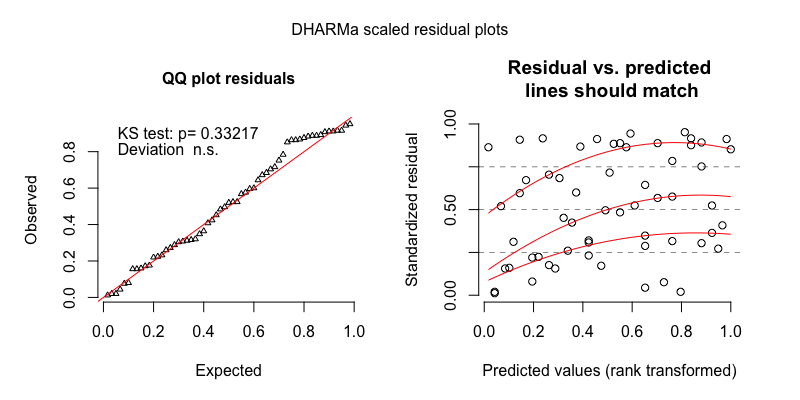
\includegraphics[width=0.9\linewidth]{www/TCDS_turntaking_nb_res_plot} 

}

\caption{The model residuals from the negative binomial mixed-effects regression of TCDS min/hr for the turn-taking sample.}\label{fig:fig5}
\end{figure}

As an alternative analysis we generated parallel models of TCDS rate in
the turn-taking clips using gaussian mixed-effects regression with
logged values of TCDS: results for the two models demonstrating all
pairwise effects of time of day are shown in
\protect\hyperlink{tab7}{Table 7} and \protect\hyperlink{tab8}{Table 8}.
The residuals for the default gaussian model
(\protect\hyperlink{tab7}{Table 7}) are shown in
\protect\hyperlink{fig6}{Figure 6}.

\FloatBarrier

\begin{table}[tbp]
\begin{center}
\begin{threeparttable}
\caption{\label{tab:tab7}Full output of the gaussian mixed-effects regression of TCDS min/hr for the turn-taking sample, with midday as the reference level for time of day.}
\begin{tabular}{llllll}
\toprule
component & \multicolumn{1}{c}{term} & \multicolumn{1}{c}{estimate} & \multicolumn{1}{c}{std.error} & \multicolumn{1}{c}{statistic} & \multicolumn{1}{c}{p.value}\\
\midrule
cond & (Intercept) & 2.40 & 0.26 & 9.41 & 0.00\\
cond & tchiyr.std & 0.09 & 0.23 & 0.37 & 0.71\\
cond & stthr.trimorning & 0.13 & 0.34 & 0.38 & 0.70\\
cond & stthr.triafternoon & 0.05 & 0.30 & 0.17 & 0.86\\
cond & hsz.std & 0.13 & 0.15 & 0.89 & 0.37\\
cond & nsk.std & -0.14 & 0.12 & -1.16 & 0.24\\
cond & tchiyr.std:stthr.trimorning & -0.17 & 0.32 & -0.52 & 0.60\\
cond & tchiyr.std:stthr.triafternoon & 0.04 & 0.27 & 0.15 & 0.88\\
cond & tchiyr.std:nsk.std & 0.07 & 0.15 & 0.49 & 0.62\\
random\_effect & aclew\_child\_id & 0.22 & NA & NA & NA\\
random\_effect & Residual & 0.71 & NA & NA & NA\\
\bottomrule
\end{tabular}
\end{threeparttable}
\end{center}
\end{table}

\begin{table}[tbp]
\begin{center}
\begin{threeparttable}
\caption{\label{tab:tab8}Model output of the gaussian mixed-effects regression of TCDS min/hr for the turn-taking sample, with afternoon as the reference level for time of day.}
\begin{tabular}{llllll}
\toprule
component & \multicolumn{1}{c}{term} & \multicolumn{1}{c}{estimate} & \multicolumn{1}{c}{std.error} & \multicolumn{1}{c}{statistic} & \multicolumn{1}{c}{p.value}\\
\midrule
cond & (Intercept) & 2.46 & 0.18 & 13.76 & 0.00\\
cond & tchiyr.std & 0.13 & 0.21 & 0.60 & 0.55\\
cond & stthr.tri.amidday & -0.05 & 0.30 & -0.17 & 0.86\\
cond & stthr.tri.amorning & 0.08 & 0.26 & 0.29 & 0.77\\
cond & hsz.std & 0.13 & 0.15 & 0.89 & 0.37\\
cond & nsk.std & -0.14 & 0.12 & -1.16 & 0.24\\
cond & tchiyr.std:stthr.tri.amidday & -0.04 & 0.27 & -0.15 & 0.88\\
cond & tchiyr.std:stthr.tri.amorning & -0.21 & 0.29 & -0.70 & 0.48\\
cond & tchiyr.std:nsk.std & 0.07 & 0.15 & 0.49 & 0.62\\
random\_effect & aclew\_child\_id & 0.22 & NA & NA & NA\\
random\_effect & Residual & 0.71 & NA & NA & NA\\
\bottomrule
\end{tabular}
\end{threeparttable}
\end{center}
\end{table}

\FloatBarrier

\begin{figure}[H]

{\centering 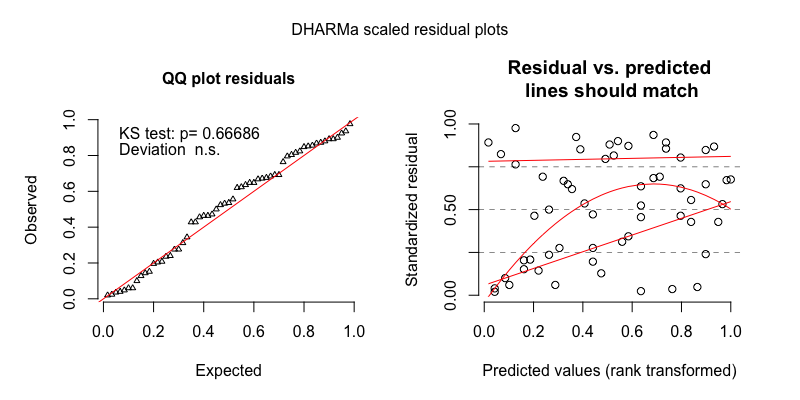
\includegraphics[width=0.9\linewidth]{www/TCDS_turntaking_log_gaus_res_plot} 

}

\caption{The model residuals from the gaussian mixed-effects regression of TCDS min/hr for the turn-taking sample.}\label{fig:fig6}
\end{figure}

\FloatBarrier

\subsection{Other-directed speech (ODS)}\label{models-ods}

\subsubsection{Random clips}\label{models-ods-random}

ODS rate in the random clips demonstrated a skewed distribution with
extra cases of zero \protect\hyperlink{fig7}{Figure 7}. We therefore
modeled it using a zero-inflated negative binomial mixed-effects
regression.in the main text: results for the two models demonstrating
all pairwise effects of time of day are shown in
\protect\hyperlink{tab9}{Table 9} and \protect\hyperlink{tab10}{Table
10}. The residuals for the default model (\protect\hyperlink{tab9}{Table
9}) are shown in \protect\hyperlink{fig8}{Figure 8}.

\FloatBarrier

\begin{figure}[H]

{\centering 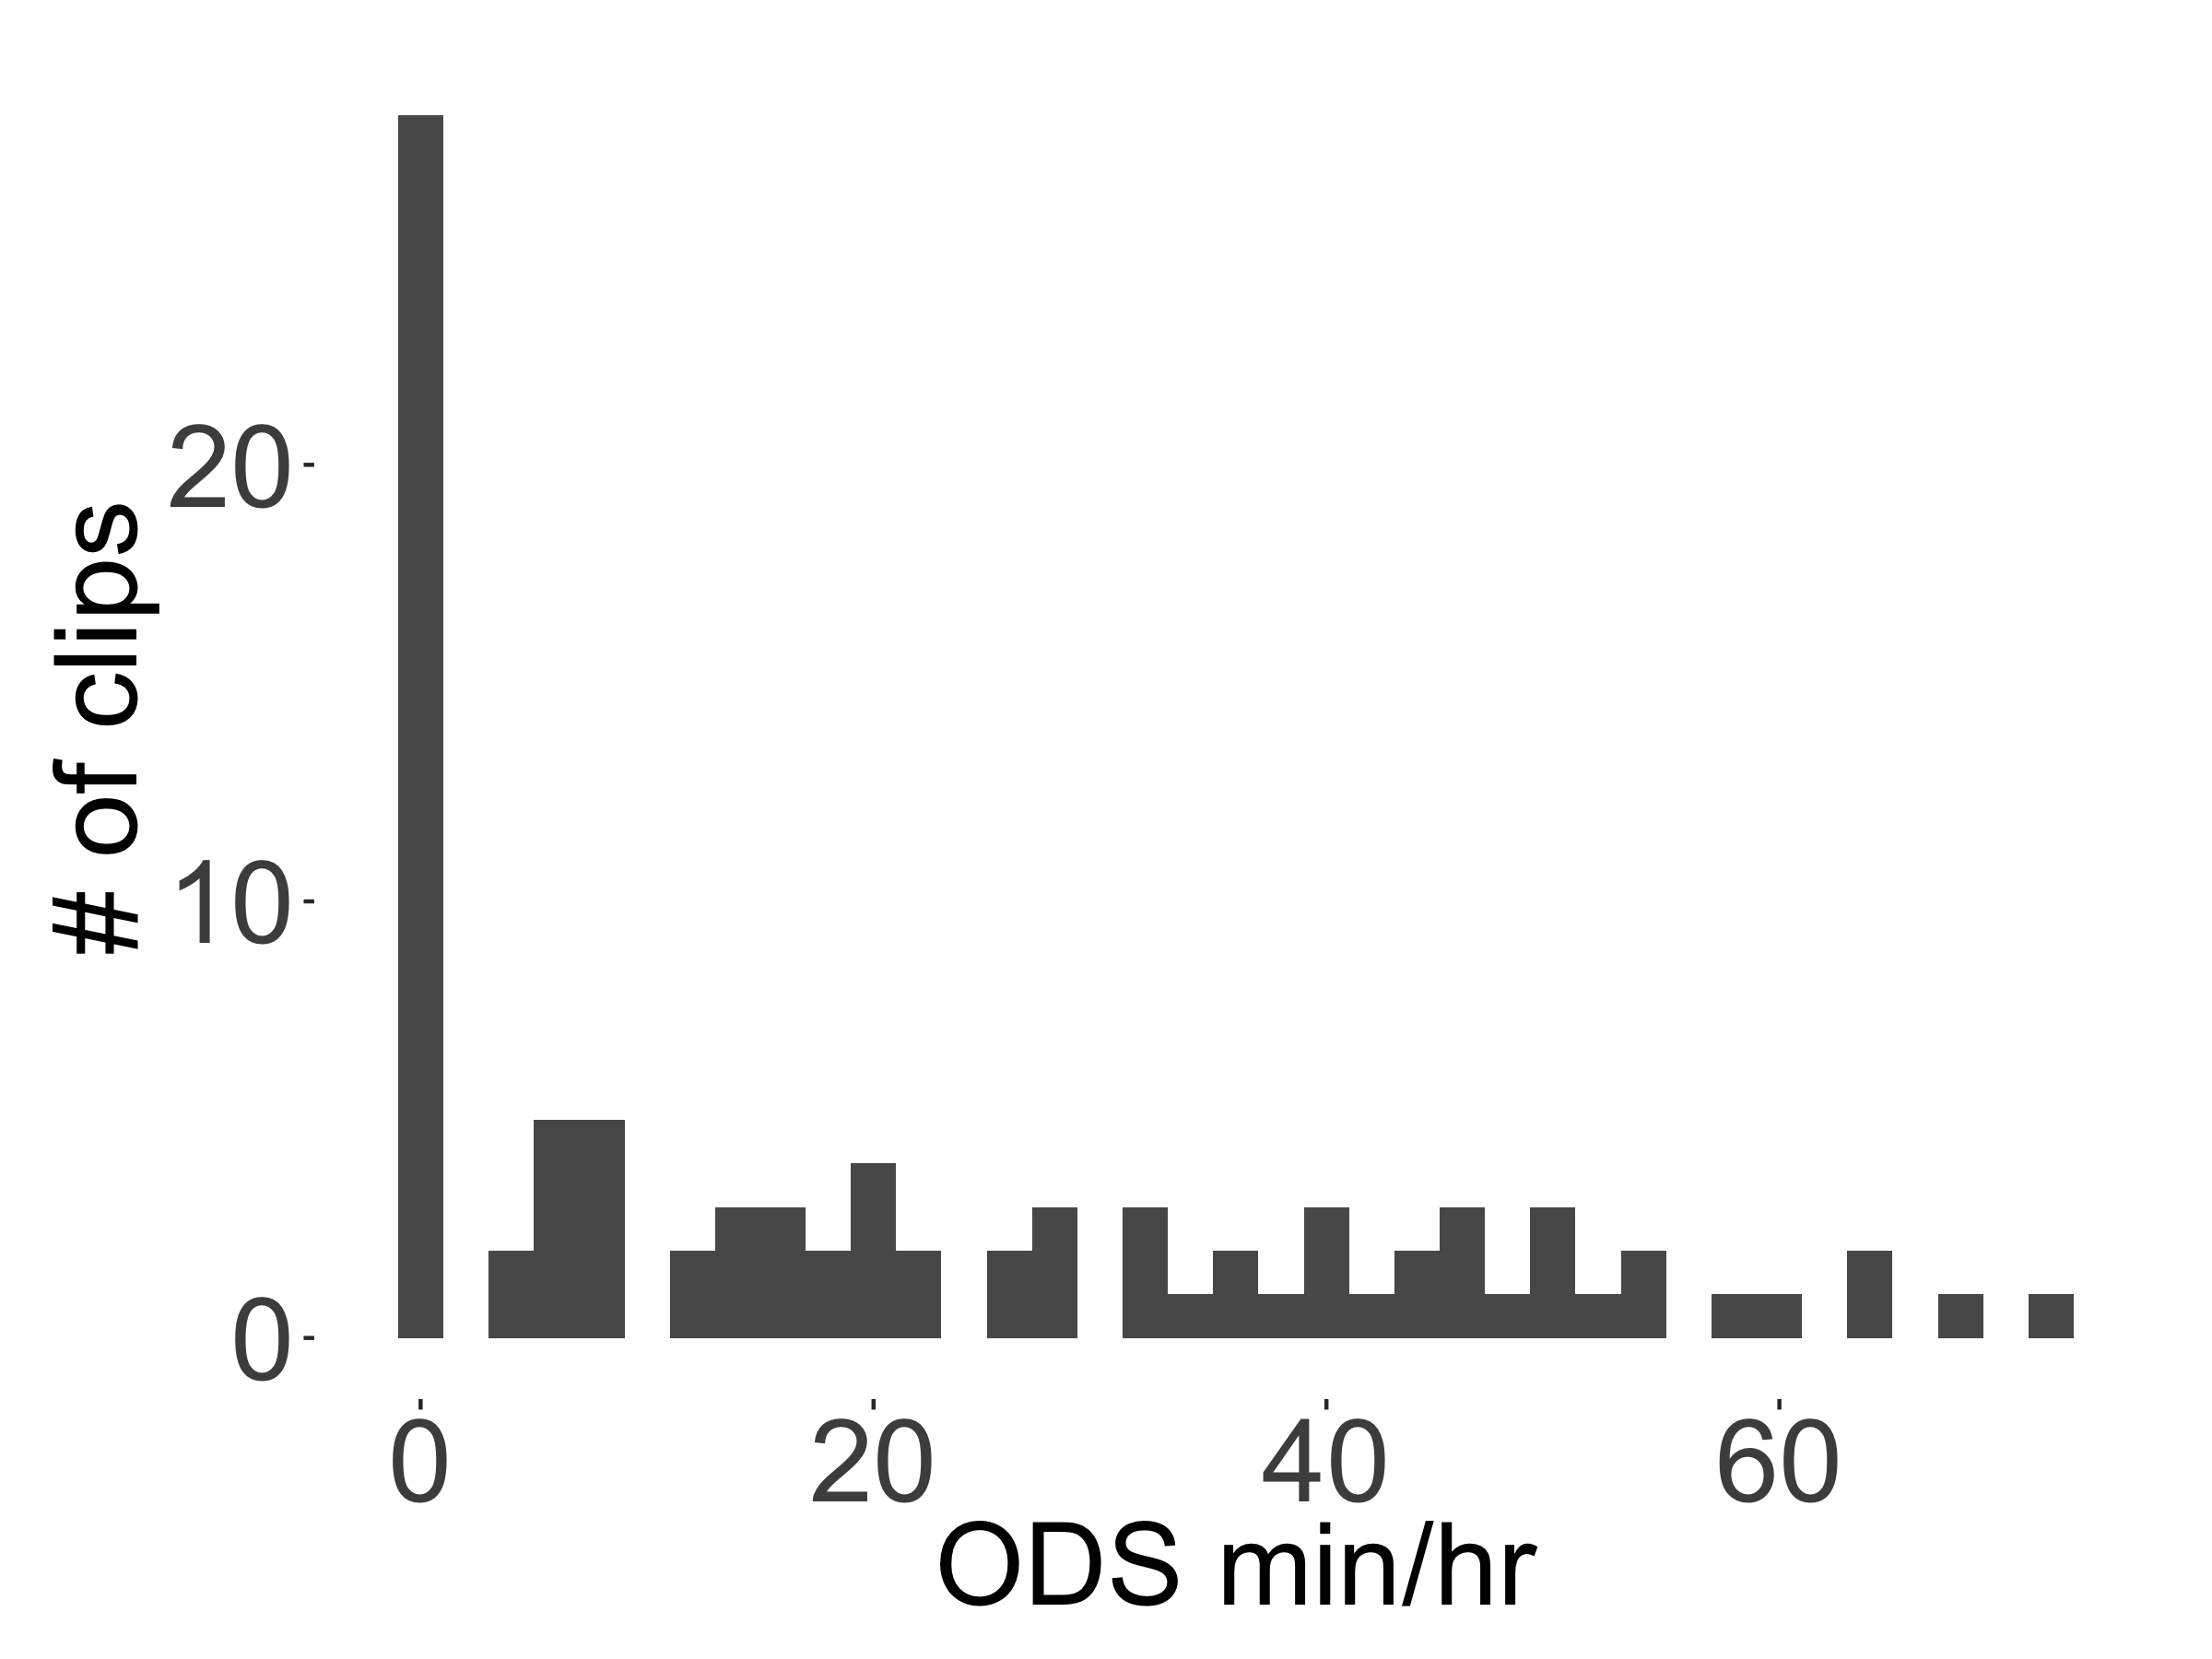
\includegraphics[width=0.4\linewidth]{www/ODS_random_distribution} 

}

\caption{The distribution of ODS rates found across the 90 random clips.}\label{fig:fig7}
\end{figure}

\FloatBarrier

\begin{table}[tbp]
\begin{center}
\begin{threeparttable}
\caption{\label{tab:tab9}Full output of the zero-inflated negative binomial mixed-effects regression of ODS min/hr for the random sample, with midday as the reference level for time of day.}
\begin{tabular}{llllll}
\toprule
component & \multicolumn{1}{c}{term} & \multicolumn{1}{c}{estimate} & \multicolumn{1}{c}{std.error} & \multicolumn{1}{c}{statistic} & \multicolumn{1}{c}{p.value}\\
\midrule
cond & (Intercept) & 2.71 & 0.16 & 16.87 & 0.00\\
cond & tchiyr.std & -0.39 & 0.16 & -2.43 & 0.02\\
cond & stthr.trimorning & 0.45 & 0.18 & 2.49 & 0.01\\
cond & stthr.triafternoon & 0.33 & 0.16 & 2.00 & 0.05\\
cond & hsz.std & -0.12 & 0.08 & -1.52 & 0.13\\
cond & nsk.std & 0.68 & 0.09 & 7.29 & 0.00\\
cond & tchiyr.std:stthr.trimorning & 0.26 & 0.20 & 1.31 & 0.19\\
cond & tchiyr.std:stthr.triafternoon & 0.42 & 0.17 & 2.42 & 0.02\\
cond & tchiyr.std:nsk.std & 0.14 & 0.11 & 1.29 & 0.20\\
zi & (Intercept) & -51.51 & 13,502.22 & 0.00 & 1.00\\
zi & nsk.std & -55.02 & 13,734.07 & 0.00 & 1.00\\
random\_effect & aclew\_child\_id & 0.00 & NA & NA & NA\\
\bottomrule
\end{tabular}
\end{threeparttable}
\end{center}
\end{table}

\begin{table}[tbp]
\begin{center}
\begin{threeparttable}
\caption{\label{tab:tab10}Model output of the zero-inflated negative binomial mixed-effects regression of ODS min/hr for the random sample, with afternoon as the reference level for time of day.}
\begin{tabular}{llllll}
\toprule
component & \multicolumn{1}{c}{term} & \multicolumn{1}{c}{estimate} & \multicolumn{1}{c}{std.error} & \multicolumn{1}{c}{statistic} & \multicolumn{1}{c}{p.value}\\
\midrule
cond & (Intercept) & 3.04 & 0.11 & 27.93 & 0.00\\
cond & tchiyr.std & 0.03 & 0.10 & 0.32 & 0.75\\
cond & stthr.tri.amidday & -0.33 & 0.16 & -2.00 & 0.05\\
cond & stthr.tri.amorning & 0.12 & 0.15 & 0.83 & 0.41\\
cond & hsz.std & -0.12 & 0.08 & -1.52 & 0.13\\
cond & nsk.std & 0.68 & 0.09 & 7.29 & 0.00\\
cond & tchiyr.std:stthr.tri.amidday & -0.42 & 0.17 & -2.42 & 0.02\\
cond & tchiyr.std:stthr.tri.amorning & -0.16 & 0.16 & -0.98 & 0.33\\
cond & tchiyr.std:nsk.std & 0.14 & 0.11 & 1.29 & 0.20\\
zi & (Intercept) & -50.05 & 10,018.85 & 0.00 & 1.00\\
zi & nsk.std & -53.54 & 10,190.89 & 0.00 & 1.00\\
random\_effect & aclew\_child\_id & 0.00 & NA & NA & NA\\
\bottomrule
\end{tabular}
\end{threeparttable}
\end{center}
\end{table}

\FloatBarrier

\begin{figure}[H]

{\centering 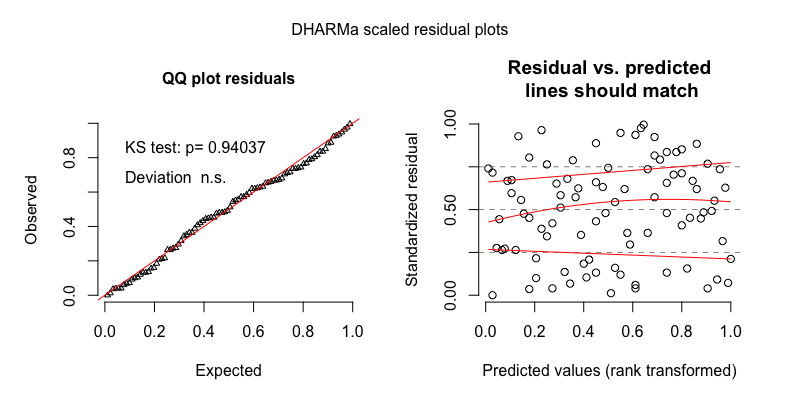
\includegraphics[width=0.9\linewidth]{www/ODS_random_z-inb_res_plot} 

}

\caption{The model residuals from the zero-inflated negative binomial mixed-effects regression of ODS min/hr for the random sample.}\label{fig:fig8}
\end{figure}

As an alternative analysis we generated parallel models of ODS rate in
the random clips using gaussian mixed-effects regression with logged
values of ODS: results for the two models demonstrating all pairwise
effects of time of day are shown in \protect\hyperlink{tab11}{Table 11}
and \protect\hyperlink{tab12}{Table 12}. The residuals for the default
gaussian model (\protect\hyperlink{tab11}{Table 11}) are shown in
\protect\hyperlink{fig9}{Figure 9}.

\FloatBarrier

\begin{table}[tbp]
\begin{center}
\begin{threeparttable}
\caption{\label{tab:tab11}Full output of the gaussian mixed-effects regression of ODS min/hr for the random sample, with midday as the reference level for time of day.}
\begin{tabular}{llllll}
\toprule
component & \multicolumn{1}{c}{term} & \multicolumn{1}{c}{estimate} & \multicolumn{1}{c}{std.error} & \multicolumn{1}{c}{statistic} & \multicolumn{1}{c}{p.value}\\
\midrule
cond & (Intercept) & 2.04 & 0.15 & 13.37 & 0.00\\
cond & tchiyr.std & -0.26 & 0.18 & -1.49 & 0.14\\
cond & stthr.trimorning & 0.23 & 0.21 & 1.09 & 0.28\\
cond & stthr.triafternoon & 0.35 & 0.19 & 1.86 & 0.06\\
cond & hsz.std & -0.38 & 0.11 & -3.37 & 0.00\\
cond & nsk.std & 1.56 & 0.10 & 16.30 & 0.00\\
cond & tchiyr.std:stthr.trimorning & 0.07 & 0.23 & 0.31 & 0.75\\
cond & tchiyr.std:stthr.triafternoon & 0.43 & 0.20 & 2.08 & 0.04\\
cond & tchiyr.std:nsk.std & 0.18 & 0.11 & 1.58 & 0.11\\
random\_effect & aclew\_child\_id & 0.00 & NA & NA & NA\\
random\_effect & Residual & 0.73 & NA & NA & NA\\
\bottomrule
\end{tabular}
\end{threeparttable}
\end{center}
\end{table}

\begin{table}[tbp]
\begin{center}
\begin{threeparttable}
\caption{\label{tab:tab12}Model output of the gaussian mixed-effects regression of ODS min/hr for the random sample, with afternoon as the reference level for time of day.}
\begin{tabular}{llllll}
\toprule
component & \multicolumn{1}{c}{term} & \multicolumn{1}{c}{estimate} & \multicolumn{1}{c}{std.error} & \multicolumn{1}{c}{statistic} & \multicolumn{1}{c}{p.value}\\
\midrule
cond & (Intercept) & 2.40 & 0.11 & 21.11 & 0.00\\
cond & tchiyr.std & 0.16 & 0.13 & 1.22 & 0.22\\
cond & stthr.tri.amidday & -0.35 & 0.19 & -1.86 & 0.06\\
cond & stthr.tri.amorning & -0.12 & 0.19 & -0.64 & 0.52\\
cond & hsz.std & -0.38 & 0.11 & -3.37 & 0.00\\
cond & nsk.std & 1.56 & 0.10 & 16.30 & 0.00\\
cond & tchiyr.std:stthr.tri.amidday & -0.43 & 0.20 & -2.08 & 0.04\\
cond & tchiyr.std:stthr.tri.amorning & -0.36 & 0.20 & -1.82 & 0.07\\
cond & tchiyr.std:nsk.std & 0.18 & 0.11 & 1.58 & 0.11\\
random\_effect & aclew\_child\_id & 0.00 & NA & NA & NA\\
random\_effect & Residual & 0.73 & NA & NA & NA\\
\bottomrule
\end{tabular}
\end{threeparttable}
\end{center}
\end{table}

\FloatBarrier

\begin{figure}[H]

{\centering 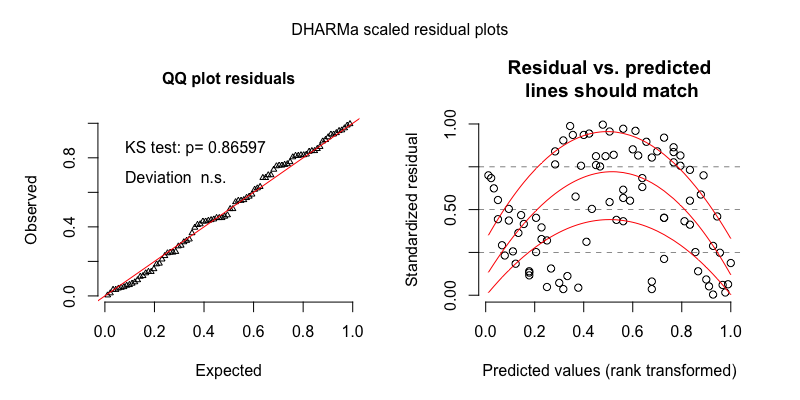
\includegraphics[width=0.9\linewidth]{www/ODS_random_log_gaus_res_plot} 

}

\caption{The model residuals from the gaussian mixed-effects regression of ODS min/hr for the random sample.}\label{fig:fig9}
\end{figure}

\FloatBarrier

\subsubsection{Turn-taking clips}\label{models-ods-turntaking}

ODS rate in the turn-taking clips demonstrated a skewed distribution
with extra cases of zero \protect\hyperlink{fig10}{Figure 10}. We
therefore modeled it using a zero-inflated negative binomial
mixed-effects regression in the main text: results for the two models
demonstrating all pairwise effects of time of day are shown in
\protect\hyperlink{tab13}{Table 13} and \protect\hyperlink{tab14}{Table
14}. The residuals for the default model
(\protect\hyperlink{tab13}{Table 13}) are shown in
\protect\hyperlink{fig11}{Figure 11}.

\FloatBarrier

\begin{figure}[H]

{\centering 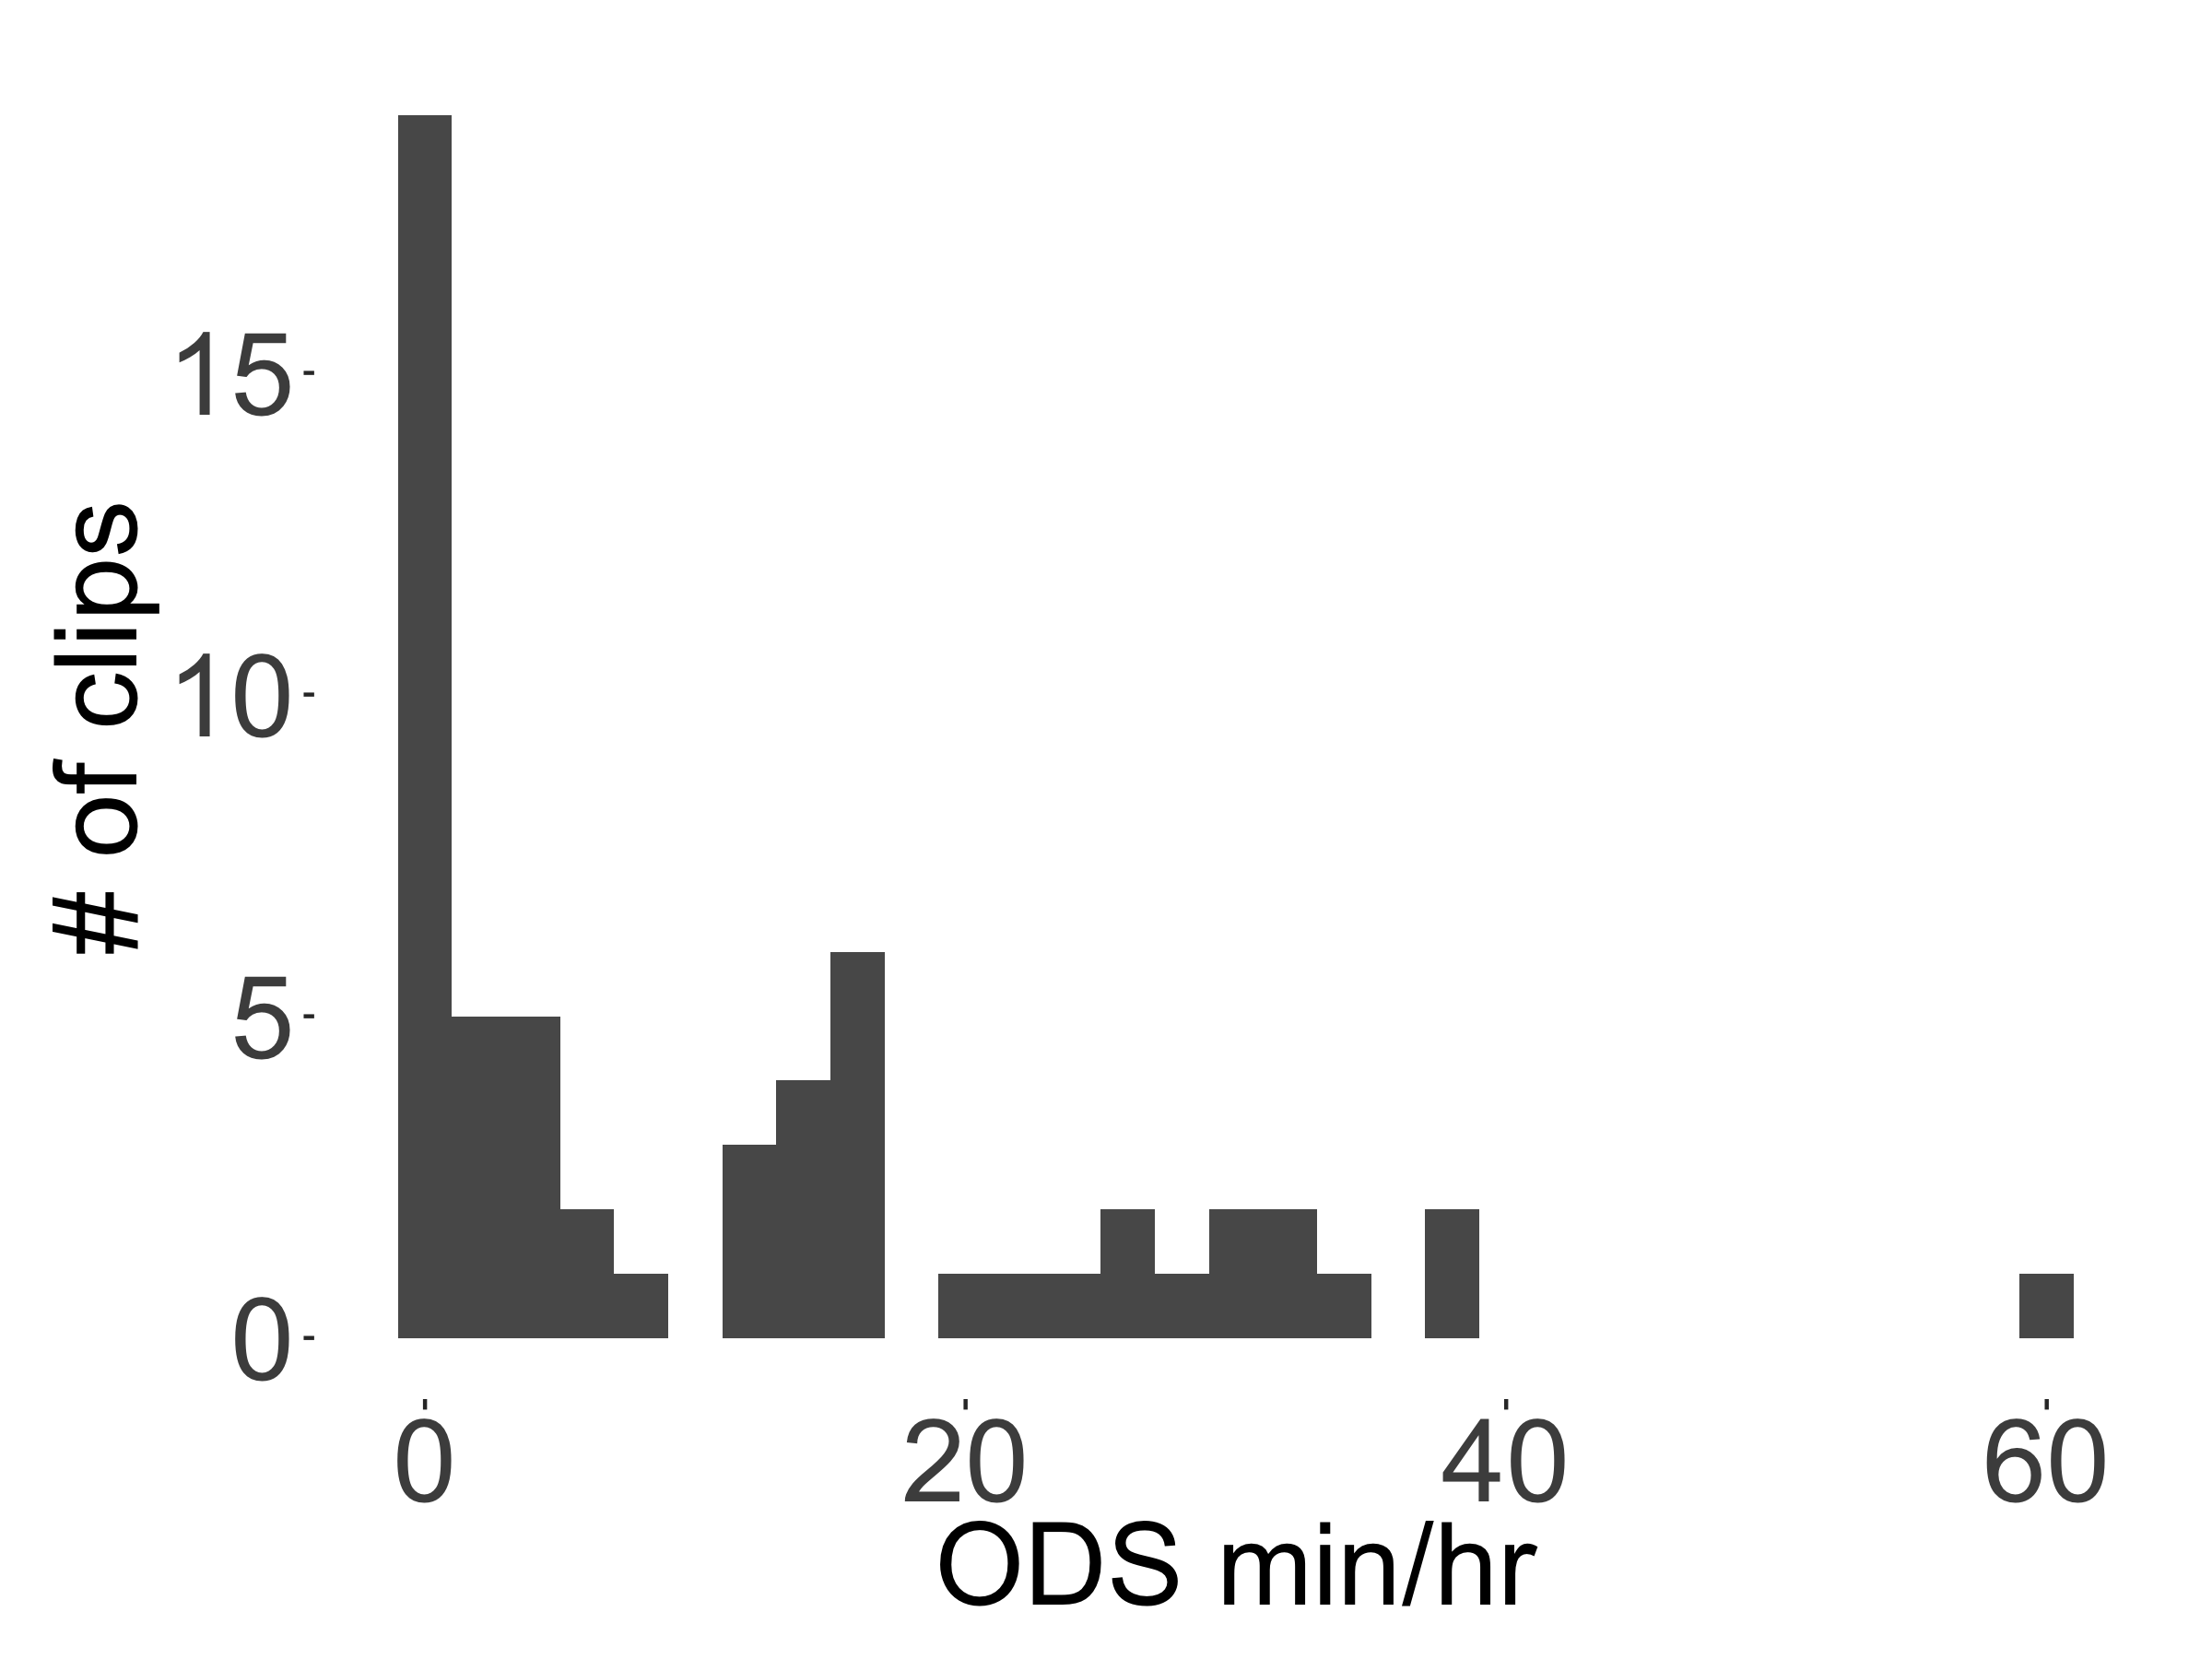
\includegraphics[width=0.4\linewidth]{www/ODS_turntaking_distribution} 

}

\caption{The distribution of ODS rates found across the 59 turn-taking clips.}\label{fig:fig10}
\end{figure}

\FloatBarrier

\begin{table}[tbp]
\begin{center}
\begin{threeparttable}
\caption{\label{tab:tab13}Full output of the negative binomial mixed-effects regression of ODS min/hr for the turn-taking sample, with morning as the reference level for time of day (note that most default models have midday as the reference level for time of day; the default model is changed here due to convergence issues).}
\begin{tabular}{llllll}
\toprule
component & \multicolumn{1}{c}{term} & \multicolumn{1}{c}{estimate} & \multicolumn{1}{c}{std.error} & \multicolumn{1}{c}{statistic} & \multicolumn{1}{c}{p.value}\\
\midrule
cond & (Intercept) & 2.64 & 0.16 & 16.02 & 0.00\\
cond & tchiyr.std & -0.80 & 0.23 & -3.43 & 0.00\\
cond & stthr.tri.oafternoon & -0.61 & 0.25 & -2.41 & 0.02\\
cond & stthr.tri.omidday & 0.00 & 0.26 & -0.01 & 0.99\\
cond & hsz.std & -0.18 & 0.09 & -2.12 & 0.03\\
cond & nsk.std & 0.63 & 0.10 & 6.44 & 0.00\\
cond & tchiyr.std:stthr.tri.oafternoon & 0.48 & 0.29 & 1.62 & 0.11\\
cond & tchiyr.std:stthr.tri.omidday & 0.54 & 0.30 & 1.77 & 0.08\\
cond & tchiyr.std:nsk.std & -0.01 & 0.14 & -0.09 & 0.93\\
zi & (Intercept) & -31.97 & 11,304.01 & 0.00 & 1.00\\
zi & nsk.std & -31.33 & 11,122.86 & 0.00 & 1.00\\
random\_effect & aclew\_child\_id & 0.00 & NA & NA & NA\\
\bottomrule
\end{tabular}
\end{threeparttable}
\end{center}
\end{table}

\begin{table}[tbp]
\begin{center}
\begin{threeparttable}
\caption{\label{tab:tab14}Model output of the negative binomial mixed-effects regression of ODS min/hr for the turn-taking sample, with afternoon as the reference level for time of day.}
\begin{tabular}{llllll}
\toprule
component & \multicolumn{1}{c}{term} & \multicolumn{1}{c}{estimate} & \multicolumn{1}{c}{std.error} & \multicolumn{1}{c}{statistic} & \multicolumn{1}{c}{p.value}\\
\midrule
cond & (Intercept) & 2.03 & 0.22 & 9.11 & 0.00\\
cond & tchiyr.std & -0.33 & 0.25 & -1.33 & 0.18\\
cond & stthr.tri.amidday & 0.61 & 0.29 & 2.07 & 0.04\\
cond & stthr.tri.amorning & 0.61 & 0.25 & 2.41 & 0.02\\
cond & hsz.std & -0.18 & 0.09 & -2.12 & 0.03\\
cond & nsk.std & 0.63 & 0.10 & 6.44 & 0.00\\
cond & tchiyr.std:stthr.tri.amidday & 0.06 & 0.31 & 0.20 & 0.84\\
cond & tchiyr.std:stthr.tri.amorning & -0.48 & 0.29 & -1.62 & 0.11\\
cond & tchiyr.std:nsk.std & -0.01 & 0.14 & -0.09 & 0.93\\
zi & (Intercept) & -32.22 & 12,257.76 & 0.00 & 1.00\\
zi & nsk.std & -31.58 & 12,061.33 & 0.00 & 1.00\\
random\_effect & aclew\_child\_id & 0.00 & NA & NA & NA\\
\bottomrule
\end{tabular}
\end{threeparttable}
\end{center}
\end{table}

\FloatBarrier

\begin{figure}[H]

{\centering 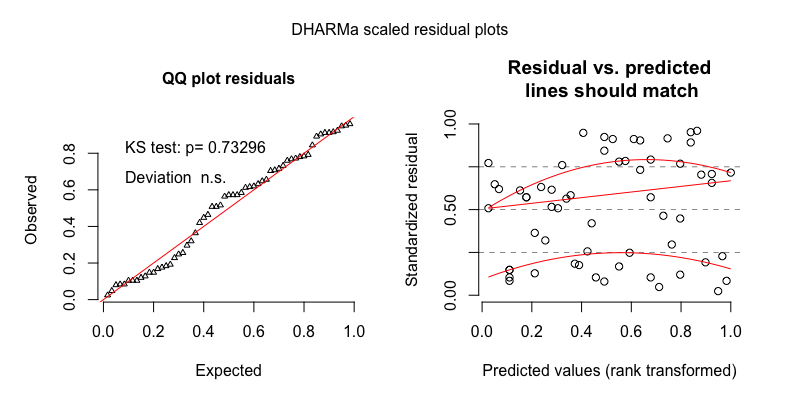
\includegraphics[width=0.9\linewidth]{www/ODS_turntaking_z-inb_res_plot} 

}

\caption{The model residuals from the zero-inflated negative binomial mixed-effects regression of ODS min/hr for the turn-taking sample.}\label{fig:fig11}
\end{figure}

As an alternative analysis we generated parallel models of ODS rate in
the turn-taking clips using gaussian mixed-effects regression with
logged values of ODS: results for the two models demonstrating all
pairwise effects of time of day are shown in
\protect\hyperlink{tab15}{Table 15} and \protect\hyperlink{tab16}{Table
16}. The residuals for the default gaussian model
(\protect\hyperlink{tab15}{Table 15}) are shown in
\protect\hyperlink{fig12}{Figure 12}.

\FloatBarrier

\begin{table}[tbp]
\begin{center}
\begin{threeparttable}
\caption{\label{tab:tab15}Full output of the gaussian mixed-effects regression of ODS min/hr for the turn-taking sample, with midday as the reference level for time of day.}
\begin{tabular}{llllll}
\toprule
component & \multicolumn{1}{c}{term} & \multicolumn{1}{c}{estimate} & \multicolumn{1}{c}{std.error} & \multicolumn{1}{c}{statistic} & \multicolumn{1}{c}{p.value}\\
\midrule
cond & (Intercept) & 2.34 & 0.21 & 10.93 & 0.00\\
cond & tchiyr.std & -0.15 & 0.20 & -0.74 & 0.46\\
cond & stthr.trimorning & -0.25 & 0.28 & -0.86 & 0.39\\
cond & stthr.triafternoon & -0.72 & 0.26 & -2.77 & 0.01\\
cond & hsz.std & -0.27 & 0.12 & -2.28 & 0.02\\
cond & nsk.std & 1.09 & 0.11 & 10.02 & 0.00\\
cond & tchiyr.std:stthr.trimorning & -0.25 & 0.29 & -0.86 & 0.39\\
cond & tchiyr.std:stthr.triafternoon & 0.06 & 0.26 & 0.23 & 0.82\\
cond & tchiyr.std:nsk.std & -0.08 & 0.14 & -0.60 & 0.55\\
random\_effect & aclew\_child\_id & 0.00 & NA & NA & NA\\
random\_effect & Residual & 0.69 & NA & NA & NA\\
\bottomrule
\end{tabular}
\end{threeparttable}
\end{center}
\end{table}

\begin{table}[tbp]
\begin{center}
\begin{threeparttable}
\caption{\label{tab:tab16}Model output of the gaussian mixed-effects regression of ODS min/hr for the turn-taking sample, with afternoon as the reference level for time of day.}
\begin{tabular}{llllll}
\toprule
component & \multicolumn{1}{c}{term} & \multicolumn{1}{c}{estimate} & \multicolumn{1}{c}{std.error} & \multicolumn{1}{c}{statistic} & \multicolumn{1}{c}{p.value}\\
\midrule
cond & (Intercept) & 1.62 & 0.16 & 10.44 & 0.00\\
cond & tchiyr.std & -0.09 & 0.19 & -0.49 & 0.62\\
cond & stthr.tri.amidday & 0.72 & 0.26 & 2.77 & 0.01\\
cond & stthr.tri.amorning & 0.47 & 0.24 & 1.94 & 0.05\\
cond & hsz.std & -0.27 & 0.12 & -2.28 & 0.02\\
cond & nsk.std & 1.09 & 0.11 & 10.02 & 0.00\\
cond & tchiyr.std:stthr.tri.amidday & -0.06 & 0.26 & -0.23 & 0.82\\
cond & tchiyr.std:stthr.tri.amorning & -0.30 & 0.27 & -1.13 & 0.26\\
cond & tchiyr.std:nsk.std & -0.08 & 0.14 & -0.60 & 0.55\\
random\_effect & aclew\_child\_id & 0.00 & NA & NA & NA\\
random\_effect & Residual & 0.69 & NA & NA & NA\\
\bottomrule
\end{tabular}
\end{threeparttable}
\end{center}
\end{table}

\FloatBarrier

\begin{figure}[H]

{\centering 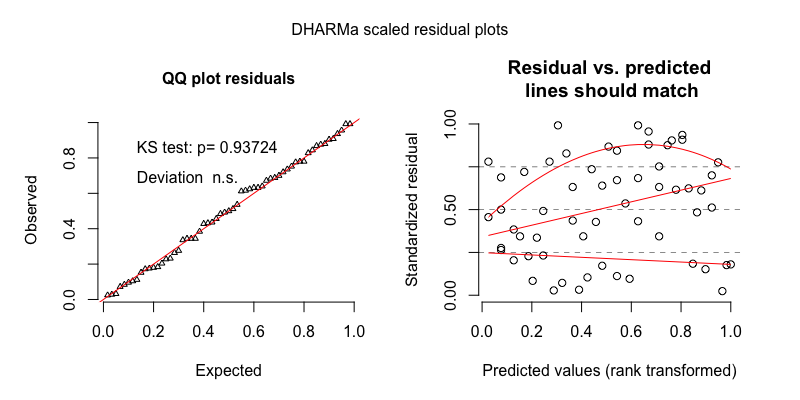
\includegraphics[width=0.9\linewidth]{www/ODS_turntaking_log_gaus_res_plot} 

}

\caption{The model residuals from the gaussian mixed-effects regression of ODS min/hr for the turn-taking sample.}\label{fig:fig12}
\end{figure}

\FloatBarrier

\section{References}\label{refs}

\begingroup
\setlength{\parindent}{-0.5in} \setlength{\leftskip}{0.5in}

\hypertarget{refs}{}
\hypertarget{ref-R-glmmTMB}{}
Brooks, M. E., Kristensen, K., van Benthem, K. J., Magnusson, A., Berg,
C. W., Nielsen, A., \ldots{} Bolker, B. M. (2017a). glmmTMB balances
speed and flexibility among packages for zero-inflated generalized
linear mixed modeling. \emph{The R Journal}, \emph{9}, 378--400.

\hypertarget{ref-brooks2017modeling}{}
Brooks, M. E., Kristensen, K., van Benthem, K. J., Magnusson, A., Berg,
C. W., Nielsen, A., \ldots{} Bolker, B. M. (2017b). Modeling
zero-inflated count data with glmmTMB. \emph{bioRxiv}.
\url{https://doi.org/10.1101/132753}

\endgroup






\end{document}
